The search for gravitational waves is not a binary process, the
instrument does not simply emit zeroes until a wave is detected, at
which time it emits a one.  We have seen in figure~\ref{f:first_stage}
of the previous chapter that even in Gaussian noise the search
produces background triggers.

In order to claim the detection of a gravitational wave we must have a
candidate whose significance stands well above that of these
background triggers.  So far this thesis has focused on increasing 
the efficiency of the search to increase the significance of the 
signals.  We now shift focus to reducing the number of triggers in the
background.  The key to doing this is ability to \emph{veto} time,
that is, remove from the analysis times which we believe will pollute
the background and/or times in which we would be unable to confidently
detect a real signal.

In this chapter we discuss the infrastructure that enables such
vetoes.  In the next chapter we look at a tool, \emph{daily ihope},
which was used in S6 to characterize the behavior of the detectors and
determine times that needed to be vetoed.


\subsection{Data Quality Flags}

The state of the instrument at any time is summarized by a set of
\emph{flags}.  Flags are identified by a triple of (ifo id, flag name,
version number), where \emph{ifo id} identifies the instrument,
\emph{flag name} is a unique identifier, and \emph{version number} is
an integer starting from 1.  The version number allows information to
be updated without losing information that may be needed to
reconstruct the results of earlier searches.  The full set of flags is
stored in a database designed at Syracuse and hosted at Caltech.

Flags are stored as a set of \emph{segments}, half-open intervals
aligned on GPS integer second boundaries.  Each flag triple has an
associated set of segments indicating the times during which it is
\emph{defined}.  Such triples also have a set of segments indicating
times during which they are \emph{active}.  The set of active segments
must be a subset of defined segments.  Times during which a flag is
defined and not active are considered \emph{inactive}.

Flags may be entered manually through a web interface.  This can be
used to indicate nonstandard operating conditions, such as heavy
equipment being operated on site.  However, most flags are generated
automatically.

The first line of defense against noise triggers is on-site as the
instrument is running.  At all such times the control room is staffed
by an operator who is an expert in running the instrument employed by
LIGO labs, and a science monitor (``SciMon'') who is a member of the
LIGO Scientific Collaboration.  The two jointly decide when to enable
\emph{science mode}, which marks the data as suitable for analysis.
This declaration is not specific to the CBC group, but extends to all
searches in the collaboration.  Science time is indicated by the flag
\texttt{DMT\_SCIENCE}.

In addition to the readout channel (\texttt{DARM\_ERR}, described in
section~\ref{sec:ligo_detectors}) many other data channels are
recorded, falling into two broad categories.  Physical environmental
monitor (``PEM'') channels record information about the environment
such as seismic activity at the base and end stations, microphones and
magnetometers placed throughout the site, etc.  Instrumental
(``INST'') channels record data from numerous subsystems such as
servos for each mirror and the output of photodiodes at points
throughout the light path.  Software running at the sites called the
data monitoring tool (``DMT'') creates data quality flags based on
these channels.  For example, when a channel's value or standard
deviation over time exceeds a given threshold.  The DMT is also
responsible for recording the state of the science mode flag.  Other
flags are set by programs that run analyses on these auxiliary
channels, for examples see~\cite{Isogai:2010}.



\iffalse
\subsection{Technical details}

The flag segments are stored in a high-performance relational
database, exposed as a web service which provides secure access to all
members of the collaboration.  Several utilities to interact with the
segment database were written, many of which could run in many modes.
The names of all these utilities start with ligolw, short for ``LIGO
lightweight,'' an XML-based format used throughout the collaboration
in which the output was generated.

Except where noted all programs accept a common subset of arguments
\begin{itemize}
\item \texttt{--gps-start-time} and \texttt{--gps-end-time}: Integer
GPS times specifying the time range over which to run.
\item \texttt{--include-segments}: Takes a comma-separated list of
segment specifiers of the form ifo:flag\_name:version or
ifo:flag\_name and restricts the query to matching flags.  In the
latter case, report on the latest version of the flag defined at each
time within the time range.
\item \texttt{--exclude-segments}: Takes a comma-separated list of
segment specifiers in the same format as \texttt{--include-segments}.
Runs a second query on the excluded segments and returns the set of
segments in included segments - (included segments $\cap$ excluded
segments).
\item \texttt{--database}, \texttt{--segment-url},
\texttt{--dmt-files}: Specifies the data source (segment database or
XML files with segment information).
\end{itemize}


The programs used during S6 were:

\textbf{ligolw\_dq\_query}.  This program reports on the state of
flags at one or more GPS times given on the command line.  This
program does not support \\
\texttt{--gps-start-time} or \texttt{--gps-end-time}.   The available modes are

\begin{itemize}
\item \texttt{--report}:  Returns the active/inactive status of all DQ flags at the
given times.  For active flags reports the start and end times of the
segment within which the given time is contained.  For inactive flags
reports the end time of the nearest preceding segment and the start
time of the nearest subsequent segment.  This mode is used in the
daily ihope ``loudest glitches'' page, see below.
\item \texttt{--defined}: Returns a list of flags defined at the
given times.
\item \texttt{--active}: Returns a list of the flags that were active
at the given times.
\item \texttt{--start-pad}, \texttt{--end-pad}: Extends the
\texttt{--defined} and \texttt{--active} modes to report on the status
of flags within a small range of time.
\end{itemize}


\textbf{ligolw\_segment\_query}.  This program reports on the state of a
set of flags over a span of times.  The available modes are

\begin{itemize}
\item \texttt{--show-types}: Reports the sets of flags that exist over
the time span.
\item \texttt{--query-types}: Reports the segments during which the
flags were defined.
\item \texttt{--query-segments}: Reports the segments during which the
flags were active.
\end{itemize}

Every CBC analysis begins by determining the science mode times with a
call of the form

\vspace*{5mm}
\texttt{ligolw\_segment\_query} \\
\hspace*{0.5in}\texttt{--query-segments --include-segments H1:DMT-SCIENCE:3 ...}
\vspace*{5mm}

\textbf{ligolw\_segments\_from\_cats}.  Given a veto definer file,
report on segments to be vetoed. 

\textbf{ligolw\_dq\_active\_cats}.  Given a veto definer file and GPS
time, report on the active/inactive status and veto category for all
flags defined at the time.

\textbf{ligolw\_segment\_insert}.  Adds new segments to the database,
enforcing various policy decisions:
\begin{itemize}
\item New segments for an existing flag/version number pair must not overlap 
with existing segments.  To update information a new version number must be used.
\item New version numbers must be one greater than the largest
existing version number.
\item New segments must not extend into the future, past the GPS time
at which the program is run.
\end{itemize}
\fi

% https://www.lsc-group.phys.uwm.edu/daswg/wiki/content_of_segment_publication_and_discovery



%%%%%%%%%%%%%%%%%%%%%%%%%%%%%%%%%
\section{Repositories for Data Quality Flags}

In order for data quality information to be used in searches and
available to investigators it must be stored in specified locations
and formats, and common creation and access tools must be available.
We must also be able to recreate the state of all flags at the time of
an analysis, in order to be able to fully vet any potential candidate
detections.  This later point implies that if a flag is updated the
old version must be maintained.

In S6 two parallel solutions were pursued:
\begin{enumerate}
\item A database-based solution allowed users to store and query segment
information. This was based on the infrastrure used in S5, updated with
the lessons learned from the science run.
\item The same tools used to query the database could be used 
to query online DQ data files generated by the DMT, simply by
changing one command-line argument. This allowed 
users to perform small low-latency queries relevant to online
searches in the most direct manner possible.
\end{enumerate}

\section{Implementation plan}

\begin{figure}[h]
  \begin{center}
    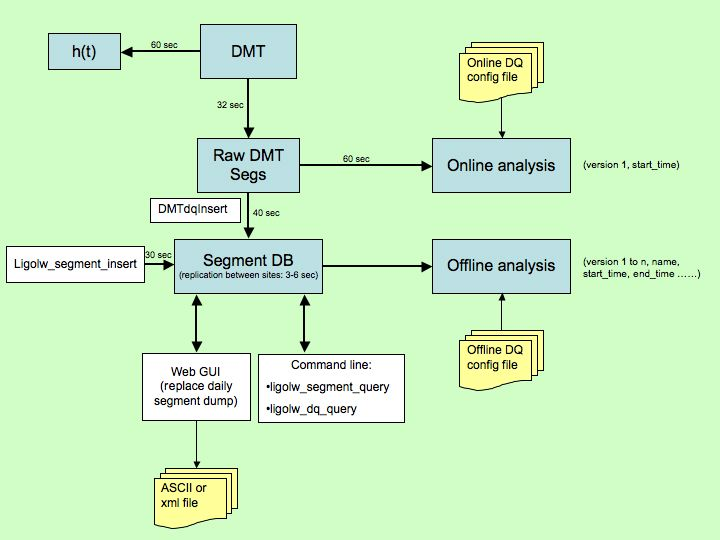
\includegraphics[width=0.9\linewidth]{figures/segdb/T0900005_fig1}
  \end{center}
  \caption[Flow of S6 data quality information]{
  Flow of S6 data quality segment information. Online data
  quality segments and science segment information is generated by the DMT.
  This can be directly queried for low-latency online analysis or inserted
  into a segment database for off-line or higher-latency analyses. Command
  line and web GUI tools were used to query and update the segment
  database.} 
\end{figure}

\begin{enumerate}
\item \textbf{DMT trigger manager:} The DMT trigger manager handled
the creation of all science segments and online data quality segments
in S6. Every 60 seconds, the DMT trigger manager wrote segment
information in XML format to disk at the Observatories. The DMT called
the \texttt{dmtdq\_seg\_insert} program to insert the XML data into
the segment database.

To prevent confusion with case sensitivity in processing tools, all
DQ flag names were required to be in upper case case. Additionally, a
3-letter prefix was be added to each DQ flag to better identify the
source where data came from. For example: the S5 DQ flag known as
\texttt{Wind\_Over\_30MPH} would be written into the XML file as
\texttt{DMT-WIND\_OVER\_30MPH} in S6. All DQ flags generated online by
the DMT had version number 1.

\item \textbf{Archival of DMT segment data:} The 60 second XML files
generated by the DMT were archived every 3600 seconds onto the LDAS
\verb|/archive/dataprods| filesystem for replication to Caltech and
Teir 2 computing centers. Files were compressed using the gzip
algorithm.

\item Software was developed to combine the segment
information from DMT XML files with a data quality categorization file
managed by the search groups (see section~\ref{sec:veto_definer}
below) to produce files containing veto information for a given search
once per minute or so.  The same software was be made available for
interfacing with the segment database for offline searches and
detector characterization (see section~\ref{ssec:from_cats}
below).

\item \textbf{Expected Latencies:} as described in the implementation plan
diagram, targeted latencies were:
\begin{itemize}
\item DMT generates h(t) file: 60 seconds
\item From DMT to raw DMT segment disk: 60 seconds
\item From raw DMT segment disk to segment database: 10 seconds
\item From ligolw\_segment\_insert to segment database: 30 seconds
\end{itemize}
\end{enumerate}



%%%%%%%%%%%%%%%%%%%%%%%%%%%%%%%%%%%%%%%%%%%%%%%%
\section{S6 segment database design}

The segment database schema (and hence the XML files) were
substantially simplified from the S5 implementations.  The five tables
to used for S6 were shown in figure~\ref{f:schema}. All unnecessary
tables were eliminated and the remaining table set simplified.
The \verb|process|, \verb|process_params| and \verb|segment_definer|
tables were unchanged from S5, with the exception that the
\verb|domain| column in the \verb|process| table was used to store the
distingished name of the user inserting the data.  In S5, segments
were either stored as on or off allowing users to distinguish between
a segment being off or undefined, due to data not being analyzed. It
was found that the off/undefined query was used substantially less
than the on query, and so in S6 this column was eliminated from the
\verb|segment| table.  To ensure that off/undefined information is
still available, the \verb|segment_summary| was introduced in S6 to
store time intervals when quality flags are defined. This further
simplified the query ``What versions were defined at what time?''
allowing better use of version information in S6.

\begin{figure}[h]
  \begin{center}
    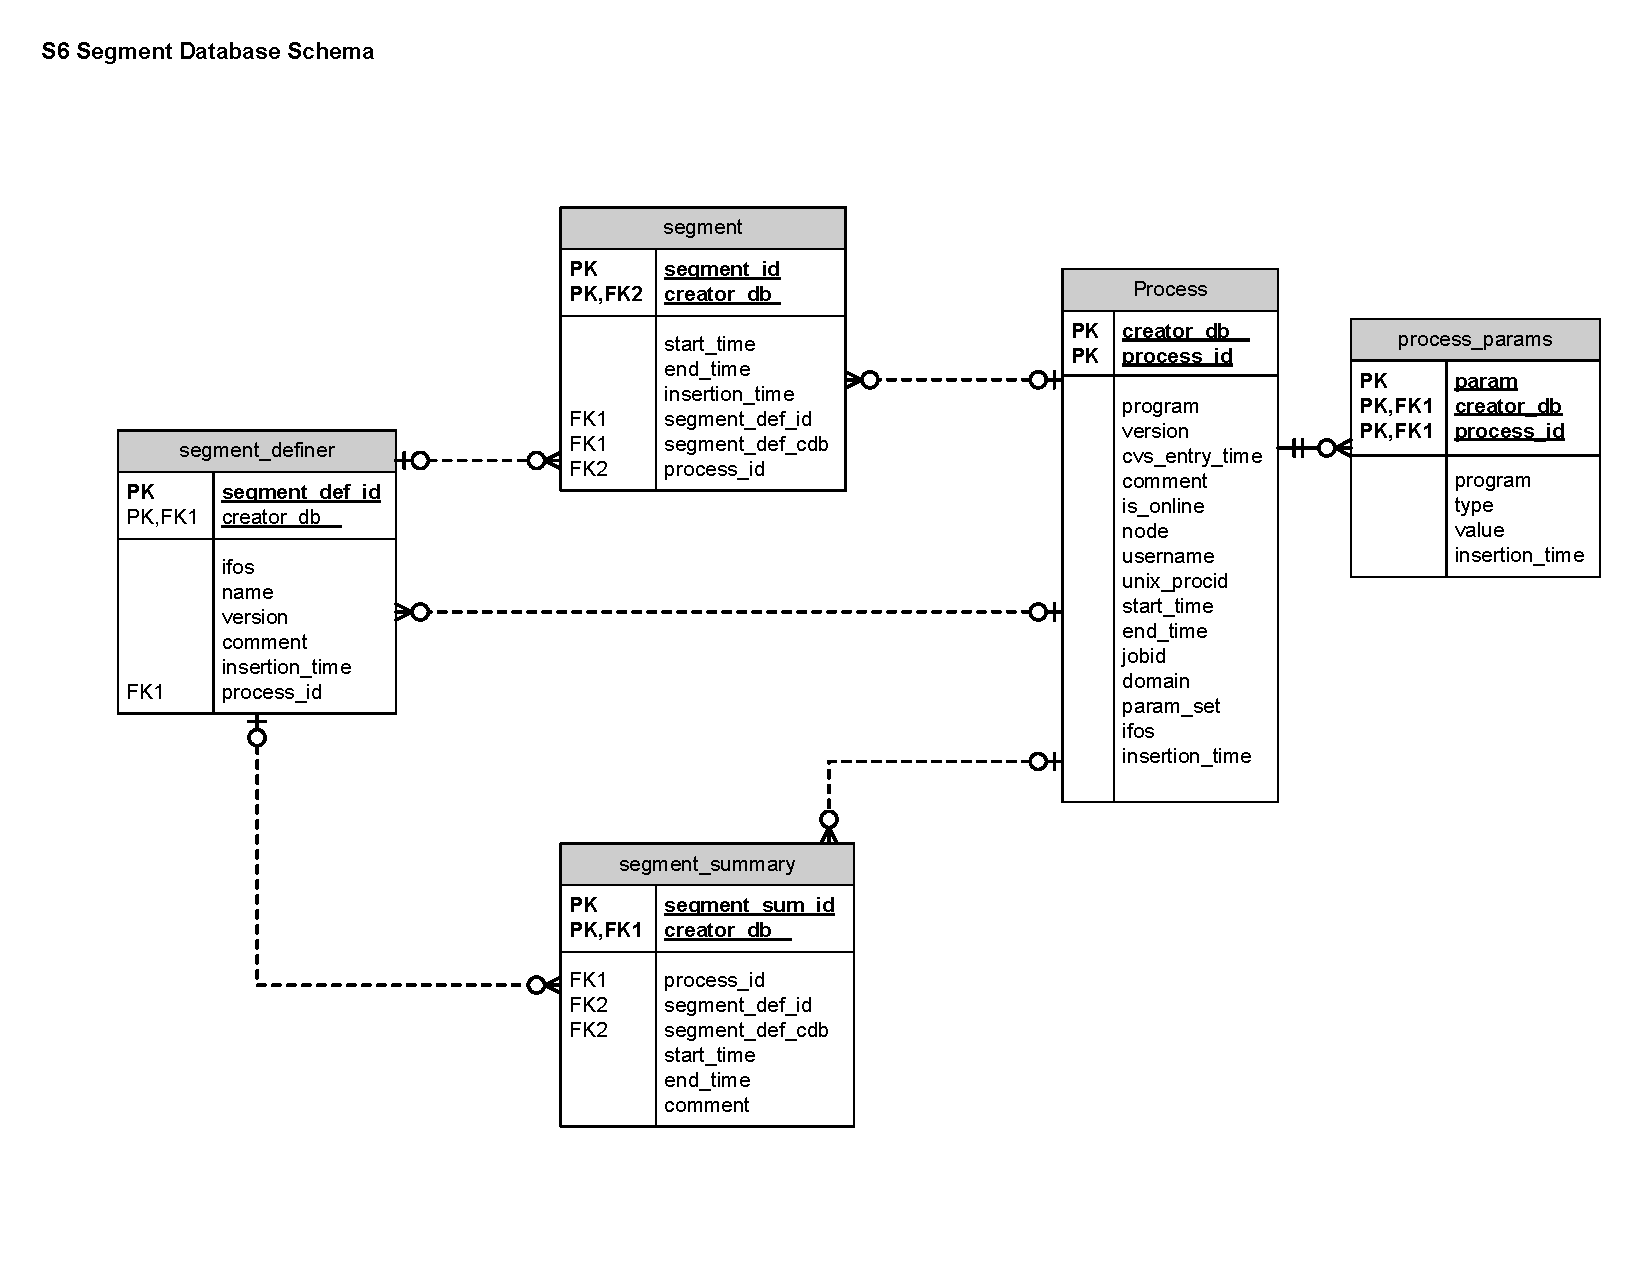
\includegraphics[width=0.9\linewidth]{figures/segdb/T0900005_fig3}
  \end{center}
  \label{f:schema}
  \caption{S6 Segment Database Schema}
\end{figure}





%%%%%%%%%%%%%%%%%%%%%%%%%%%%%%%%%%%%%%%%%%%%%%%%
\section{Data Replication Between Observatories and Tier 2 Centers}

In S6, the Caltech segment database was the official data repository.
In addition to being written into the database, all data inserted in
to the Caltech segment database was output as XML files to a
central location. These XML files were then replicated to tier 2
sites at ldas.ligo-wa.caltech.edu, ldas.ligo-la.caltech.edu. A rsync
script was implemented at Caltech to periodically replicate XML
files from Caltech to tier 2 sites.  


%%%%%%%%%%%%%%%%%%%%%%%%%%%%%%%%%%%%%%%%%%%%%%%%%
\section{Command Line Tools}

Several utilities were created that allowed user to query the segment
database and XML files.

\subsubsection{ligolw\_segment\_query}

The program \verb|ligolw_segment_query| replaced the S5
\verb|LSCsegFind| as the command line interface to query for data
quality and science segments.  \verb|ligolw_segment_query| only provided
read access to the segment database.  \verb|ligolw_segment_query|
was primarily intended for human interaction with the segment database.
Automated generation of DQ files for online searches used the
program \verb|ligolw_veto_segments|.

Below are the questions that \texttt{ligolw\_segment\_query} was
designed to answer:

\begin{itemize}
\item What DQ flags exist in the database?
\texttt{ligolw\_segment\_query --show-types}
\item When was a given flag inserted? \texttt{ligolw\_segment\_query
--query-types}
\item When was a given DQ flag defined? \texttt{ligolw\_segment\_query
--query-types}
\item When was a given flag active? \texttt{ligolw\_segment\_query
--query-segments}
\end{itemize}

The built-in help message, generated by \texttt{ligolw\_segment\_query
--help} is shown below:

DESCRIPTION:
{\small
\begin{verbatim}
  --version             show program's version number and exit
  -h, --help            show this help message and exit
  -p, --ping            Ping the target server
  -y, --show-types      Returns a xml table containing segment type
                        information: ifos, name, version,
                        segment_definer.comment, segment_summary.start_time,
                        segment_summary.end_time, segment_summary.comment
  -u, --query-types     Returns a ligolw document whose segment_definer table
                        includes all segment types defined in the given period
                        and included by include-segments and whose
                        segment_summary table indicates the times for which
                        those segments are defined.
  -q, --query-segments  Returns a ligolw document whose segment table contains
                        the times included by the include-segments flag and
                        excluded by exclude-segments
  -s gps_start_time, --gps-start-time=gps_start_time
                        Start of GPS time range
  -e gps_end_time, --gps-end-time=gps_end_time
                        End of GPS time range
  -t segment_url, --segment-url=segment_url
                        Segment URL. Users have to specify either 'https://'
                        for a secure connection or 'http://' for an insecure
                        connection in the segment database url. For example,
                        '--segment-url=https://segdb.ligo.caltech.edu'. No
                        need to specify port number.
  -d, --database        use database specified by environment variable
                        S6_SEGMENT_SERVER. For example,
                        'S6_SEGMENT_SERVER=https://segdb.ligo.caltech.edu'
  -f, --dmt-files       use files in directory specified by environment
                        variable ONLINEDQ, for example,
                        'ONLINEDQ=file:///path_to_dmt'. 'file://' is the
                        prefix, the acutal directory to DMT xml files starts
                        with '/'.
  -a include_segments, --include-segments=include_segments
                        This option expects a comma separated list of a colon
                        separated sublist of interferometer, segment type, and
                        version. The union of segments from all types and
                        versions specified is returned. Use --show-types to
                        see what types are available.   For example:
                        --include-segment-types H1:DMT-SCIENCE:1,H1:DMT-
                        INJECTION:2 will return the segments for which H1 is
                        in either SCIENCE version 1 or INJECTION version 2
                        mode. If version information is not provided, the
                        union of the segments of the latest version of
                        requested segment type(s) will be returned.
  -b exclude_segments, --exclude-segments=exclude_segments
                        This option has to be used in conjunction with
                        --include-segment-types --exclude-segment-types
                        subtracts the union of unwanted segments from the
                        specified types from the results of --include-segment-
                        types. If version information is not provided,
                        --exclude-segment-types subtracts the union of
                        segments from the latest version of the specified
                        segment types. For example, --include-segment-types H1
                        :DMT-SCIENCE:1,H1:DMT-INJECTION:2 --exclude-segment-
                        types H1:DMT-WIND:1,H1:DMT-NOT_LOCKED:2,H2:DMT-
                        NOT_LOCKED:2 will subtract the union of segments which
                        H1 is in version 1 WIND and H1,H2 is version 2
                        NOT_LOCKED from the result of --include-segment-types
                        H1:DMT-SCIENCE:1,H1:DMT-INJECTION:2
  -S, --strict-off      The default behavior is to truncate segments so that
                        returned segments are entirely in the interval [gps-
                        start-time, gps-end-time).  However if this option is
                        given, the entire non-truncated segment is returned if
                        any part of it overlaps the interval.
  -o output_file, --output-file=output_file
                        File to which output should be written.  Defaults to
                        stdout.
\end{verbatim}
}

\subsubsection{ligolw\_dq\_query}

\texttt{ligolw\_dq\_query} could query either the segment database or directories
containing XML segment files generated by the DMT.
\texttt{ligolw\_dq\_query}
only provided read access to the segment database. 

Below are the questions that \texttt{ligolw\_dq\_query} was designed
to answer:

\begin{itemize}
\item is a given flag active at a given time?
\texttt{ligolw\_dq\_query --active}
\item is a given flag defined at a given time?
\texttt{ligolw\_dq\_query --defined}
\item what is the status of all flags at a given time?
\texttt{ligolw\_dq\_query --report}
\end{itemize}


The built-in help message, generated by \texttt{ligolw\_dq\_query
--help} is shown below:

DESCRIPTION:
{\small
\begin{verbatim}
  --version             show program's version number and exit
  -h, --help            show this help message and exit
  -p, --ping            Ping the target server
  -y, --defined         Returns a segment summary table containing segments
                        defined at the given time(s).
  -u, --active          Returns a segment table containing segments active at
                        the given time(s).
  -q, --report          Prints which flags are defined/undefined at the given
                        time(s). For the flags which were defined, it
                        determines if the flag was active or inactive at that
                        time. For an active flag, it prints the start and end
                        time of the segment to which the active. For an
                        inactive flag, it prints the end time of the previous
                        adjacent active segment and the start time of the next
                        adjacent active segment
  -s start_pad, --start-pad=start_pad
                        Seconds before given time(s) to include in query
  -e end_pad, --end-pad=end_pad
                        Seconds after given time(s) to include in query
  -t segment_url, --segment-url=segment_url
                        Segment URL
  -d, --database        use database specified by environment variable
                        S6_SEGMENT_SERVER
  -f, --dmt-files       use files in directory specified by environment
                        variable ONLINEDQ
  -a include_segments, --include-segments=include_segments
                        This option expects a comma separated list of a colon
                        separated sublist of interferometer, segment type, and
                        version. The union of segments from all types and
                        versions specified is returned. Use --show-types to
                        see what types are available.   For example:
                        --include-segment-types H1:SCIENCE:1,H1:INJECTION:2
                        will return the segments for which H1 is in either
                        SCIENCE version 1 or INJECTION version 2 mode. If
                        version information is not provided, the union of the
                        segments of the latest version of requested segment
                        type(s) will be returned.
  -o output_file, --output-file=output_file
                        File to which output should be written.  Defaults to
                        stdout.
  -i, --in-segments-only
                        If set, report will only return segments that given
                        times were within
\end{verbatim}
}



\subsubsection{ligolw\_segments\_from\_cats}
\label{ssec:from_cats}

\texttt{ligolw\_segments\_from\_cats} read a veto definer file (see
section~\ref{sec:veto_definer}) and accessed either segment XML files
or the segment database in order to produce a list of times to be
vetoed.  The built-in help message is displayed below:

DESCRIPTION:
\begin{verbatim}
  --version             show program's version number and exit
  -h, --help            show this help message and exit
  -v veto_file, --veto-file=veto_file
                        veto XML file (required).
  -o output_dir, --output-dir=output_dir
                        Directory to write output (default=cwd).
  -k, --keep-db         Keep sqlite database.
  -t segment_url, --segment-url=segment_url
                        Segment URL
  -d, --database        use database specified by environment variable
                        S6_SEGMENT_SERVER
  -f, --dmt-file        use files in directory specified by environment
                        variable ONLINEDQ
  -c, --cumulative-categories
                        If set the category N files will contain all segments
                        in categories <= N
  -p, --separate-categories
                        If set the category N files will contain only category
                        N
  -s gps_start_time, --gps-start-time=gps_start_time
                        Start of GPS time range
  -e gps_end_time, --gps-end-time=gps_end_time
                        End of GPS time range
\end{verbatim}


For example:
\begin{alltt}
ligolw\_segments\_from\_cats
  --gps-start-time 930960015
  --gps-end-time 931564887
  --segment-url https://segdb.ligo.caltech.edu:30015
  --cumulative-categories
  --veto-file H1L1V1-S6\_CBC\_LOWMASS\_ONLINE-928271454-0.xml
\end{alltt}




\subsubsection{ligolw\_segment\_insert}

\texttt{ligolw\_segment\_insert} was the replacement for S5's 
LSCdqInsert.   It handled two tasks:

\begin{itemize}
\item Insert segments and/or segment types into the segment database.
\item Append segments to the existing segment types.
\end{itemize}

The built-in help message is displayed below:

DESCRIPTION:
\begin{verbatim}
  -h, --help            show this help message and exit
  -p, --ping            Ping the target server
  -t URL, --segment-url=URL
                        Users have to specify protocol 'https://' for a secure
                        connection in the segment database url. For example,
                        '--segment-url=https://segdb.ligo.caltech.edu'. No
                        need to specify port number'.
  -o FILE, --output=FILE
                        Write segments to FILE rather than the segment
                        database
  -j IDENTITY, --identity=IDENTITY
                        Set the subject line of the server's service
                        certificate to IDENTITY
  -I, --insert          Insert segments to the segment database
  -A, --append          Append segments to an existing segment type
  -i IFOS, --ifos=IFOS  Set the segment interferometer to IFOS (e.g. H1)
  -n NAME, --name=NAME  Set the name of the segment to NAME (e.g. DMT-
                        BADMONTH)
  -v VERSION, --version=VERSION
                        Set the numeric version of the segment to VERSION
                        (e.g. 1)
  -e EXPLAIN, --explain=EXPLAIN
                        Set the segment_definer:comment to COMMENT. This
                        should explaining WHAT this flag mean (e.g. "Light dip
                        10%"). Required when --Insert/-I is specified.
  -c COMMENT, --comment=COMMENT
                        Set the segment_summary:comment to COMMENT. This
                        should explaining WHY these segments were inserted
                        (e.g. "Created from hveto results")
  -S FILE, --summary-file=FILE
                        Read the segment_summary rows from FILE. This should
                        be a file containing the gps start and end times that
                        the flag was defined, deliminated by comma (i.e. the union of on and off)
  -G FILE, --segment-file=FILE
                        Read the segment rows from FILE. This should containin
                        the gps start and end times when the flag was active deliminated by comma
\end{verbatim}

As an example, the command to insert segments of a new type would 
look like:

\begin{alltt}
ligolw\_segment\_insert
  --segment-url https://segdb.ligo.caltech.edu
  --ifos 'H1'
  --name 'DCH-TEST'
  --version 1
  --comment 'testing if insert works'
  --explain 'test insert'
  --segment-file segment.txt
  --summary-file summary.txt
  --insert
\end{alltt}

To append segments to an existing segment, the command would look like:

\begin{alltt}
ligolw\_segment\_insert 
  --segment-url https://segdb.ligo.caltech.edu
  --ifos 'H1'
  --name 'DCH-TEST'
  --version 1
  --comment 'testing if append works'
  --segment-file append\_segment.txt
  --summary-file append\_summary.txt
  --append
\end{alltt}

%%%%%%%%%%%%%%%%%%%%%%%%%%%%%%%%%%%%%%%%%%%%%%%%%%
\section{Functionality Supported in S6}
With the above described infrastructure and command line tools
users were able to determine

\begin{itemize}
\item When was a given flag defined?
\item Was a given flag defined at this time?
\item When was a given flag active?
\item What is the dead time for a given flag? 
\item At a given point of time, is the given flag active? If yes, find
out the start and end time of the segment to which the specified point
of time belongs.
\item At a given point of time, is the given flag active? If no, find
out the end time of the previous adjacent active segment and the start
time of the next adjacent active segment.
\item Provide the same supports described above for a set of flags.
\item What flags were active at this time, near this time ($\pm 1$~s
interval or specified by user)?
\item What is the efficiency for a flag for burst and inspiral and
plot it.
\item Export answer to ascii or xml file
\item Handle padding windows for deadtime queries
\item Export config files, start, end times
\end{itemize}


%%%%%%%%%%%%%%%%%%%%%%%%%%%%%%%%%%%%%%%%%%%%%%%%%
\section{Authentication}

In S6, data insertion requires authentication. Retrieving from on-site
requires no authentication. Retrieving from off-site requires
authentication.  The authentication system is beyond the scope of this
document.

\section{Segment Data File Format}

To be ingested into the segment database, segment data must be in the
format described in this section. Data should be in a valid LIGO LW
XML file with \verb|process|, \verb|segment_definer|,
\verb|segment_summary| and \verb|segment| tables. An optional
\verb|process_params| table can be used to store extra metadata about
segment generation.

The \verb|process| table should contain the columns given in the XML
file below which describe the name, version, cvs repository and
revision of the program used generate the data. The comment column can
be used to add additional human-readable data. The node, username,
unix\_procid, start\_time and end\_time columns should store metadata
describing who ran the process and where it ran. The ifos column
should contain an alphabetical list of all ifo data using as input to
the process. The process\_id column is used to link the defined
process to other rows in the file created by that process.

The \verb|segment_definer| table should contain a definition of the
segments included in the file. The ifos, name and version column
should contain the name and version of the segment. The name should be
upper case for all segments. DMT-derived segments should be prefixed
with the string \verb|DMT-|, Kleinewelle derived veto segments should
be prefixed with the string \verb|KWV-|, data derived from the
detector state vector channels should be prefixed with \verb|IFO-|,
segments created by the detchar group should be prefixes with
\verb|DCH-| and segments from the Virgo database should be prefixed
with \verb|VDB-|.  The comment column can be used to add a
human-readable description of the segment. The segment\_definer column
is used to link this type of segment to the intervals in the
\verb|segment| and \verb|segment_summary| tables.

The \verb|segment| table should contain the GPS start and end time
when the segment described in the \verb|segment_definer| table was
\emph{active}. The \verb|segment_summary| table should contain the GPS
start time and end time of the interval for which the segment is
\emph{defined}. This will allow users to distinguish between the cases
where a DQ segment is undefined for a particular time or simply
inactive (i.e. it is \emph{not} windy, as opposed to the wind monitor
being down).

{\tiny
\begin{verbatim}
<?xml version="1.0"?>
<!DOCTYPE LIGO_LW SYSTEM "http://ldas-sw.ligo.caltech.edu/doc/ligolwAPI/html/ligolw_dtd.txt">
<LIGO_LW>
  <Table Name="processgroup:process:table">
    <Column Name="processgroup:process:program" Type="lstring"/>
    <Column Name="processgroup:process:version" Type="lstring"/>
    <Column Name="processgroup:process:cvs_repository" Type="lstring"/>
    <Column Name="processgroup:process:cvs_entry_time" Type="int_4s"/>
    <Column Name="processgroup:process:comment" Type="lstring"/>
    <Column Name="processgroup:process:node" Type="lstring"/>
    <Column Name="processgroup:process:username" Type="lstring"/>
    <Column Name="processgroup:process:unix_procid" Type="int_4s"/>
    <Column Name="processgroup:process:start_time" Type="int_4s"/>
    <Column Name="processgroup:process:end_time" Type="int_4s"/>
    <Column Name="processgroup:process:process_id" Type="ilwd:char"/>
    <Column Name="processgroup:process:ifos" Type="lstring"/>
    <Stream Name="processgroup:process:table" Type="Local" Delimiter=",">
      "SegGener","1.17",
      "/ldcg_server/common/repository_gds/gds/Monitors/SegGener/SegGener.cc\,v",
      865755895,"Segment generation from an OSC condition","granite","jzweizig",718,
      918756928,918836992,"process:process_id:0","H0H1H2"
    </Stream>
  </Table>
  <Table Name="segment_definergroup:segment_definer:table">
    <Column Name="segment_definergroup:segment_definer:process_id" Type="ilwd:char"/>
    <Column Name="segment_definergroup:segment_definer:segment_def_id" Type="ilwd:char"/>
    <Column Name="segment_definergroup:segment_definer:ifos" Type="lstring"/>
    <Column Name="segment_definergroup:segment_definer:name" Type="lstring"/>
    <Column Name="segment_definergroup:segment_definer:version" Type="int_4s"/>
    <Column Name="segment_definergroup:segment_definer:comment" Type="lstring"/>
    <Stream Name="segment_definergroup:segment_definer:table" Type="Local" Delimiter=",">
      "process:process_id:0","segment_definer:segment_def_id:35","H2","DMT-LIGHT",1,
      "H2 Light in arms from h(t) DQ flags",
      "process:process_id:0","segment_definer:segment_def_id:36","H2","DMT-SCIENCE",1,
      "H2 Science mode from h(t) DQ flags",
      "process:process_id:0","segment_definer:segment_def_id:37","H2","DMT-INJECTION",1,
      "H2 Injection mode from h(t) DQ flags",
      "process:process_id:0","segment_definer:segment_def_id:38","H2","DMT-UP",1,
      "H2 calibration OK in from h(t) DQ flags",
      "process:process_id:0","segment_definer:segment_def_id:39","H2","DMT-CALIBRATED",1,
      "H2 Calibration OK from h(t) DQ flags",
      "process:process_id:0","segment_definer:segment_def_id:40","H2","DMT-BADGAMMA",1,
      "H2 Bad gamma in h(t) DQ flags"
    </Stream>
  </Table>
  <Table Name="segmentgroup:segment:table">
    <Column Name="segmentgroup:segment:segment_id" Type="ilwd:char"/>
    <Column Name="segmentgroup:segment:start_time" Type="int_4s"/>
    <Column Name="segmentgroup:segment:end_time" Type="int_4s"/>
    <Column Name="segmentgroup:segment:segment_def_id" Type="ilwd:char"/>
    <Column Name="segmentgroup:segment:process_id" Type="ilwd:char"/>
    <Stream Name="segmentgroup:segment:table" Type="Local" Delimiter=",">
      "segment:segment_id:15",918836961,918836977,"segment_definer:segment_def_id:35",
      "process:process_id:0",
      "segment:segment_id:16",918836976,918836992,"segment_definer:segment_def_id:37",
      "process:process_id:0"
    </Stream>
  </Table>
  <Table Name="segment_summarygroup:segment_summary:table">
    <Column Name="segment_summarygroup:segment_summary:segment_sum_id" Type="ilwd:char"/>
    <Column Name="segment_summarygroup:segment_summary:start_time" Type="int_4s"/>
    <Column Name="segment_summarygroup:segment_summary:end_time" Type="int_4s"/>
    <Column Name="segment_summarygroup:segment_summary:comment" Type="lstring"/>
    <Column Name="segment_summarygroup:segment_summary:segment_def_id" Type="ilwd:char"/>
    <Column Name="segment_summarygroup:segment_summary:process_id" Type="ilwd:char"/>
    <Stream Name="segment_summarygroup:segment_summary:table" Type="Local" Delimiter=",">
      "segment_summary:segment_sum_id:5",918836976,918836992,"",
      "segment_definer:segment_def_id:40","process:process_id:0",
      "segment_summary:segment_sum_id:6",918836976,918836992,"",
      "segment_definer:segment_def_id:39","process:process_id:0",
      "segment_summary:segment_sum_id:11",918836976,918836992,"",
      "segment_definer:segment_def_id:37","process:process_id:0",
      "segment_summary:segment_sum_id:12",918836976,918836992,"",
      "segment_definer:segment_def_id:35","process:process_id:0",
      "segment_summary:segment_sum_id:42",918836976,918836992,"",
      "segment_definer:segment_def_id:36","process:process_id:0",
      "segment_summary:segment_sum_id:46",918836976,918836992,"",
      "segment_definer:segment_def_id:38","process:process_id:0"
    </Stream>
  </Table>
</LIGO_LW>
\end{verbatim}
}

\subsection{The Veto Definer}
\label{sec:veto_definer}

Problems in the data may have differing levels of severity, and
consequently we define several \emph{veto categories} to characterize
them.  We defer discussion of the meaning of these categories until
the next chapter, but note here that the categories are indicated by
integers from 1 to 4, in decreasing levels of severity.  We also note
that time marked with category 1 is entirely excluded form the
analysis.  4091 seconds of data with one second of category 1 time in
the middle will be split into two 2045-second chunks.  Neither of
these will be analyzable, as ihope requires 2048 seconds of data in
order to computer the PSD.  Short category 1 vetos can therefore
effectively veto much larger times, and such vetoes are therefore to
be avoided whenever possible. 

In order to veto a chunk of time it is necessary to map a data quality
flag to a veto category.  This is accomplished with a \emph{veto
definer file}.  Such files are specific to each search, as time that
is problematic for one search may pose no issues for another.  The
\texttt{ligolw\_segments\_from\_cats} program (see above) merges the
information in this file with the set of active flag segments to
produce \emph{veto segments} at each veto level.  Analysis is
performed on times marked as science with no CAT1 vetoes.  Triggers
from times marked as CAT2, CAT3 and CAT4 are discarded from both
foreground and background.

Sometimes the threshold on a DQ flag is such that the data is
unsuitable for analysis close to, but outside, the range of the flag.
The veto definer file therefore allows for \emph{padding}, offsets 
which effectively extend the flags.

\subsection{Example Veto Configuration File}

The veto configuration file should contain a \verb|process| table
describing how it was created and a \verb|veto_definer| table
describing the flags to be applied at different levels. The comment
column of the process table should contain the version of the file.
The columns in the \verb|veto_definer| table are as follows:
\verb|ifo|, \verb|name| and \verb|version| uniquely define a
particular DQ/veto flag. \verb|category| described which veto category
it should be applied at (i.e. $0, 1, 2, 3, \ldots$), \verb|start_time|
and \verb|end_time| denote the GPS time interval for which the DQ/veto
flag should be applied (Note: if \verb|end_time| is zero, then the
current GPS time is assumed). \verb|start_pad| and \verb|end_pad| are
the padding time (in seconds) applied to the start and end of the veto
segments. Note that these are signed: if you want time vetoed to start
time to be \emph{earlier} than the start time listed in the database,
then the emph \verb|start_pad| should be \emph{negative}. Similarly,
if the time vetoed should extend \emph{after} the end time stored in
the database, then the value in \verb|end_pad| should be
\emph{positive}. The \verb|comment| column can be used to store an
optional human-readable comment.

{\tiny
\begin{verbatim}
<?xml version='1.0' encoding='utf-8' ?>
<!DOCTYPE LIGO_LW SYSTEM "http://ldas-sw.ligo.caltech.edu/doc/ligolwAPI/html/ligolw_dtd.txt">
<LIGO_LW>
   <Table Name="process:table">
      <Column Name="process:process_id" Type="ilwd:char"/>
      <Column Name="process:program" Type="lstring"/>
      <Column Name="process:version" Type="lstring"/>
      <Column Name="process:cvs_repository" Type="lstring"/>
      <Column Name="process:cvs_entry_time" Type="int_4s"/>
      <Column Name="process:node" Type="lstring"/>
      <Column Name="process:username" Type="lstring"/>
      <Column Name="process:unix_procid" Type="int_4s"/>
      <Column Name="process:start_time" Type="int_4s"/>
      <Column Name="process:end_time" Type="int_4s"/>
      <Column Name="process:ifos" Type="lstring"/>
      <Column Name="process:comment" Type="lstring"/>
      <Stream Name="process:table" Type="Local" Delimiter=",">
      "process:process_id:0","ligolw_veto_file","1.1",
      "/usr/local/cvs/lscsoft/glue/bin/ligolw_veto_file,v",822908378,
      "ldas-grid.ligo.caltech.edu","jrsmith",16830,822879594,822879594,
      "H1","Example file by Josh"
      </Stream>
   </Table>
   <Table Name="veto_definer:table">
      <Column Name="veto_definer:process_id" Type="ilwd:char"/>
      <Column Name="veto_definer:ifo" Type="lstring"/>
      <Column Name="veto_definer:name" Type="lstring"/>
      <Column Name="veto_definer:version" Type="int_4s"/>
      <Column Name="veto_definer:category" Type="int_4s"/>
      <Column Name="veto_definer:start_time" Type="int_4s"/>
      <Column Name="veto_definer:end_time" Type="int_4s"/>
      <Column Name="veto_definer:start_pad" Type="int_4s"/>
      <Column Name="veto_definer:end_pad" Type="int_4s"/>
      <Column Name="veto_definer:comment" Type="lstring"/>
      <Stream Name="veto_definer:table" Type="Local" Delimiter=",">
      "process:process_id:0","H1","OUT_OF_LOCK",0,1,917985615,0,0,0,"",
      "process:process_id:0","H1","BADGAMMA",1,1,917985615,0,0,0,"",
      "process:process_id:0","H1","ASC_Overflow",0,2,917985615,0,-8,8,"ASC saturations are cat2",
      "process:process_id:0","H1","PD_Overflow",0,2,917985615,0,-8,8,"PD saturations are cat2",
      "process:process_id:0","H1","SEVERE_LSC_OVERFLOW",0,2,917985615,0,-8,8,"LSC saturations are cat2",
      "process:process_id:0","H1","INJECTION",1,2,917985615,0,-16,64,"Remove HW injections at cat1",
      "process:process_id:0","H1","ASC_Overflow",0,3,917985615,0,-8,25,"ASC saturations are cat3 with larger pad",
      "process:process_id:0","H1","SEVERE_LSC_OVERFLOW",0,3,917985615,0,-8,25,"LSC saturations are cat3 with larger pad",
      "process:process_id:0","H1","PD_Overflow",0,3,917985615,0,-8,25,"PD saturations are cat3 with larger pad",
      "process:process_id:0","H1","Wind_over_30MPH",0,3,917985615,0,-8,8,"Windy",
      "process:process_id:0","H1","LIGHTDIP_1_PERCENT",0,3,917985615,0,-2,2,"Exclude all lightdip segments",
      "process:process_id:0","H1","PRE_LOCKLOSS_10_SEC",0,3,917985615,0,0,0,"",
      "process:process_id:0","H1","PRE_LOCKLOSS_30_SEC",0,3,917985615,0,0,0,"",
      "process:process_id:0","H1","PRE_LOCKLOSS_60_SEC",0,3,917985615,0,0,0,"",
      "process:process_id:0","H1","PRE_LOCKLOSS_120_SEC",0,3,917985615,0,0,0,"",
      "process:process_id:0","H1","ASI_CORR_OVERFLOW",0,4,917985615,0,-8,25,"Does this make sense for DC readout",
      "process:process_id:0","H1","LSC_OVERFLOW",0,4,917985615,0,-8,25,"LSC saturations",
      "process:process_id:0","H1","PRE_LOCKLOSS_600_SEC",0,4,917985615,0,0,0,"",
      "process:process_id:0","H1","PRE_LOCKLOSS_1800_SEC",0,4,917985615,0,0,0,""
      </Stream>
   </Table>
</LIGO_LW>
\end{verbatim}
}


